\documentclass[a4paper,10pt]{article}
\usepackage[utf8]{inputenc}
\usepackage[spanish]{babel}
\usepackage{color}
\usepackage{graphicx}
\graphicspath{ {src/} }

\newcommand{\red}[1]{\textcolor{red}{#1}}

%opening
\title{Topic 1: Internet architecture and addressing}
\author{Albert Ribes}

\begin{document}

\maketitle

\begin{abstract}
\begin{itemize}
  \item Las respuestas en \red{rojo} son las que me hago persolnales para entenderlas bien.

  \item Las respuestas oficiales están normal
\end{itemize}
\end{abstract}

% \section

\begin{enumerate}
  %1
  \item \textbf{Explica el rol y misión que tienen los RIR en la arquitectura de Internet. Indica cuantos y
que RIR’s operan. Explica el rol que tienen los LIR en la arquitectura de Internet. Indica que
relación hay entre un AS (Autonomous System) y un RIR y entre un AS y un LIR.}

\red{
RIR: Regional Internet Registry. Son las 5 redes que hay en el mundo: ARIN, LACNIC, AFRINIC, RIPE APNIC. Agrupan a los sistemas autónomos (AS). Son organizaciones independientes que apoyan la coordinación de recursos de Internet en una zona geográfica y desarrollan políticas consistentes y promocionan las buenas prácticas en Internet
}

\red{
LIR: Local Internet Registry. Son los miembros de los RIR. Los RIR distribuyen el espacio de direcciones IP a las LIR, y son estas últimas las que lo distribuyen a los usuarios finales.
}

\red{
Una NIR sería una National Internet Registry. Coordina las direcciones IP a nivel nacional. No hay ninguna en Europa, pero sí que hay en APNIC y LACNIC
}

\red{
Se puede considerar un AS a cualquiera que use el protocolo BGP. Puesto que dentro de una RIR se habla con BGP, todos los miembros han de usar BGP, y por lo tanto todos los miembros de un RIR son AS
}




  %2
  \item \textbf{A partir de la figura siguiente, explica la arquitectura de Internet y los distintos elementos
que participan en dicha arquitectura, así como, el modelo general de negocio de dicha arquitectura}

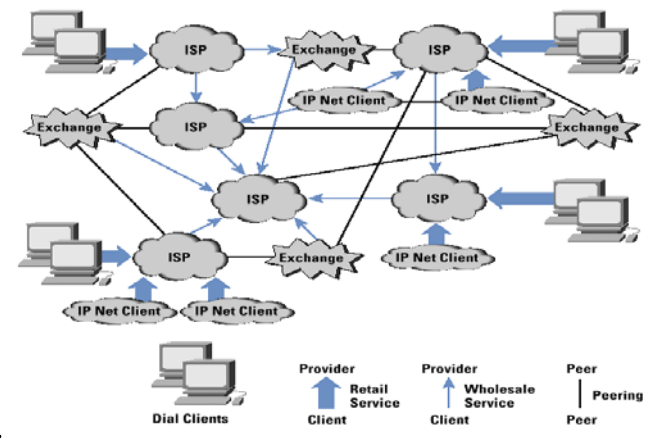
\includegraphics{p2}

  %3
  \item \textbf{Explica para que sirve una CDN (Content Distribution Network) y explica su
funcionamiento.}

  %4
  \item \textbf{Explica que es un punto neutro y quien lo compone. Explica que es la matriz de peering
de un punto neutro.¿Qué condiciones hay que cumplir para ser miembro de un punto neutro?}

  %5
  \item \textbf{Define que es un SLA (Service Level Agreement). Indica aquellos parámetros que
normalmente pueden formar parte de un SLA. ¿Qué ocurre si el ISP no cumple con alguno de los
parámetros que aparecen en el SLA? ¿Y si es el usuario o red corporativa?}

  %6
  \item \textbf{Explica que representa el Cono de Clientes (“Customer Cone”) respecto a las direcciones
IPv4 y los AS y para que se utiliza. Ilústralo con un ejemplo. ¿Qué diferencia hay entre el cono de
clientes de un AS y su grado en la representación mediante un grafo donde los vértices son los
AS’s y las aristas son las relaciones entre AS’s?}

  %7
  \item \textbf{Define e indica que representa el cono de clientes (“Customer Cone”) respecto a las
direcciones IPv4 y los AS. Dibuja una nueva figura respecto a la figura de abajo, con el nuevo
cono de clientes si (i) A y B (A es proveedor de B) cambian su relación a “A y B tienen una relación
de peer to peer”, (ii) A y B (A es proveedor de B) cambian su relación a “B es proveedor de A”.
Indica cual es el ``peering cone size ratio'' para el AS B en el caso de la figura y en los casos (i) y (ii).}

  %8
  \item \textbf{¿Qué es un Sistema Autónomo (AS)? ¿Qué diferencia hay entre usar inter-domain e intradomain routing en un AS? Explica los tipos de relaciones que tienen los AS’s.}

  %9
  \item \textbf{En una relación BGP, ¿Qué rutas anuncia un ISP cliente a su proveedor?, ¿Y el proveedor a
su cliente? ¿Y de par a par de transito? ¿Y de par a par de no-transito?}

  %10
  \item \textbf{Explica las diferencias entre las direcciones PA (Provider Aggregatable) y PI (Provider
Independent). ¿Qué ventaja desde el punto de vista de encaminamiento proporciona
el uso de direcciones PA a los ISP’s?. ¿Puede un RIR asignar redes IPv4 /22 del tipo
PI?. Justifica tu respuesta.}

  %11
  \item \textbf{Explica como funciona el mecanismo de opciones de IPv6. Explica justificadamente si
es mas eficiente usar IPv6 en un router que usar IPv4}
\end{enumerate}

\end{document}
